\documentclass[xcolor=table]{beamer}
\usepackage[utf8]{inputenc}
\usepackage[T1]{fontenc}
\usepackage[alf]{abntex2cite}	
\usepackage{udesc}
\usepackage{amsfonts,amsmath,amssymb,mathtools}
\usepackage{verbatim}
\usepackage{listings}
\usepackage[ddmmyyyy]{datetime}
\usepackage{hyperref, url}
\usepackage{graphicx}
\usepackage{multirow}
\usepackage{changepage}

\setbeamertemplate{frametitle continuation}{}

% suprimindo warnings do hyperref
\pdfstringdefDisableCommands{%
  \def\\{}%
  \def\texttt#1{<#1>}%
  \def\smallskip{}%
  \def\medskip{}%
}

\lstset{language=C++,
    basicstyle=\ttfamily,
    keywordstyle=\color{blue}\ttfamily,
    stringstyle=\color{red}\ttfamily,
    commentstyle=\color{gray}\ttfamily,
    morecomment=[l][\color{magenta}]{\#}
}

\renewcommand{\figurename}{Figura}
\sloppy
\title[]{Trabalho Final de Programação Paralela - Paralelizando Quebra de Chaves do Algoritmo RSA}

\author[Miguel Alfredo Nunes]{
    Miguel Alfredo Nunes\\\smallskip
    \texttt{miguel.alfredo.nunes@gmail.com}
}

\date{\today}

\begin{document}
    
    \begin{frame}
        \titlepage
    \end{frame}

    \begin{frame}[allowframebreaks]{Sumário}
        \tableofcontents
    \end{frame}

    \section[]{Algoritmo RSA}
    \begin{frame}{Algoritmo RSA}
        \begin{itemize}
            \item<1-> Sistema criptográfico de chave pública, qualquer um com a chave pública consegue cifrar, 
                    porém apenas a chave privada consegue decifrar;
            \item<2-> RSA: Ron \textbf{Rivest}, Adi \textbf{Shamir}, e Leonard \textbf{Adleman}
            \item<3-> História do algoritmo, segundo a Wikipedia:
                \begin{itemize}
                    \item[-]<4-> Entre 1976 e 1977 Rivest, Shamir e Adleman tentaram desenvolver uma função que calculasse números, 
                                mas que era difícil de inverter;%, ou seja, obter a entrada a partir da saída;
                    \item[-]<5-> Em abril de 1977 eles passaram o feriado de Páscoa Judaica na casa de um aluno;
                    \item[-]<6-> Lá, eles consumiram ``uma quantidade generosa de vinho'' antes de voltar para casa;
                    \item[-]<7-> Rivest, sem conseguir dormir, deitou no seu sofá com um livro de matemática - pela manhã ele tinha
                                formalizado o algoritmo.
                \end{itemize}
        \end{itemize}
    \end{frame}
    
    \begin{frame}{Algoritmo RSA}
        \begin{enumerate}
            \item Gerar aleatoriamente números primos \textit{P} e \textit{Q}, diferentes entre si;
            \item Calcular \(N = P \times Q\);
            \item Calcular um número \textit{E} que não tenha divisores em comum com \((P-1) \times (Q-1)\);
            \item Calcular um número \textit{D} tal que o resto da divisão de \(E \times D\) por \((P-1) \times (Q-1)\) é igual a 1
            \begin{itemize}
                \item[--] \textit{D} é dito inverso modular de \textit{E} modulo \((P-1) \times (Q-1)\)
            \end{itemize}        
        \end{enumerate}
        O par \(\langle E, N \rangle\) compõe a chave pública, \(\langle D, N \rangle\) compõe a chave privada.
    \end{frame}

    \begin{frame}{Algoritmo RSA}
        \begin{itemize}
            \item Sendo \textit{m} uma mensagem representada numericamente (por exemplo o código ASCII de uma letra).
            \begin{itemize}
                \item[-] Cifrar: \(m^{E}\);
                \item[-] Decifrar: \(m^{D}\);
                \item[-] \((m^{E})^{D} \equiv (m^{D})^{E} \equiv m\ (\mathtt{mod}\ N)\);
                \item[-] \((m^{D})^{E} \equiv m\ (\mathtt{mod}\ N)\) quer dizer que o resto da divisão de
                        \((m^{D})^{E}\) por \textit{N} é igual a \textit{m}.
            \end{itemize}
            \item Fatorando \textit{N} nos seus componente \textit{P} e \textit{Q} e tendo o valor \textit{E}, é fácil obter \textit{D};
            \item Segurança da criptografia se dá pela dificuldade em fazer isso - problema da fatoração de primos;
            \item Trabalho final da matéria de Complexidade de Algoritmos (CAL).
        \end{itemize}
    \end{frame}

    \section[]{Implementação}
    \begin{frame}{Implementação}
        \begin{itemize}
            \item C++ usando OpenMP, MPI e Gnu Multi Precision (GMP) - biblioteca para trabalhar com números de tamanho arbitrário;
            \item Um processo gera as chaves serialmente, são salvas em arquivos que são lidos pelo processo que vai fatorar paralelamente;
            \item Ideia principal é, dado \textit{N}, calcular os intervalos:
            \(\left[3,\left(\frac{\sqrt{N}}{x}\right)\right), \left[\left(\frac{\sqrt{N}}{x}\right), 2\times\left(\frac{\sqrt{N}}{x}\right)\right), \dots,
            \left[\left(\frac{\sqrt{N}}{x}\right)\times (x-1), \sqrt{N}\right)\) onde \textit{x} é o número de tarefas;
        \end{itemize}
    \end{frame}
    
    \begin{frame}{Implementação}
        \begin{itemize}
            \item Para obter os resultados aqui apresentados, foi executado em 8 processos que se comunicam pelo MPI, cada um com 8 threads do OpenMP;
            \item Tomando \(x = \text{processos} \times \text{threads} \times 8\), algoritmo executou sobre 512 intervalos;
            \item OpenMP e MPI não sabem como tratar os tipos do GMP, logo tive que encapsular os intervalos em uma struct e passar
                    essa struct para funções que lidam com números do GMP;
            \item Não foi possível utilizar MPI para fazer comunicação entre diversos computadores, 8 processos rodando em \texttt{localhost}.
        \end{itemize}
    \end{frame}

    \begin{frame}[fragile]{Implementação}
        \begin{lstlisting}[language=C++]
typedef struct
{
    std::string lower;
    std::string upper;
    std::string valorP;
    std::string valorQ;
}block;
        \end{lstlisting}
        \begin{itemize}
            \item GMP tem funções que traduzem números de/para strings de C, tipo \texttt{string} do C++ tem métodos para converter
                    de/para strings de C;
        \end{itemize}
    \end{frame}

    \begin{frame}[fragile]{Implementação}
        \begin{itemize}
            \item Ideia original era calcular os intervalos e comunicar um array de \texttt{block}s por MPI para todos os processos;
            \item Isso gerou muitos problemas, solução alternativa foi paralelizar a computação dos intervalos --
                cada processo calcula apenas uma porção dos intervalos:

        \begin{lstlisting}
int turn = 0;
for(int i = 1; i < total_blocos; i++){
    if(turn == PROCS)
        turn = 0;
    if(rank != turn){
        turn++;
        continue;
    }
    // calcula o intervalo
    turn++;
}
        \end{lstlisting}
        \end{itemize}
    \end{frame}

    \begin{frame}[fragile]{Implementação}
        \begin{lstlisting}
if(rank == 0)
    inicio = clock();
#pragma omp parallel
{// REGIAO PARALELA
    #pragma omp single
    {// criando tasks
        for(auto & bloco: dados){
        #pragma omp task
        {
            forcabruta_paralelo(&bloco,N, rank);
        }
        }
    }// fim do single, executando as tasks
}// FIM DA REGIAO PARALELA
if(rank == 0)
    termino = clock();
        \end{lstlisting}
    \end{frame}

    \begin{frame}[fragile]{Implementação}
        \begin{adjustwidth}{-1cm}{}
            \begin{lstlisting}
int forcabruta_paralelo(block * bloco, mpz_t N, 
    int rank){

// tira os dados do bloco

// testa um por um os numeros do limite 
// inferior ao limite superior do bloco
    if(mpz_divisible_p(N, FatorTestado) != 0){
        // calcula outro fator

        DONE = 1; // global
        MPI_Bcast(&DONE, 1, MPI_INT, rank, 
            MPI_COMM_WORLD);
        // comunica todos os processos que terminou
    }
}
            \end{lstlisting}
        \end{adjustwidth}
    \end{frame}

    \section[]{Desempenho}
    \begin{frame}{Tempos de Execução Serial}
        \begin{adjustwidth}{-1cm}{}
            \begin{figure}[htbp]
                \centering
                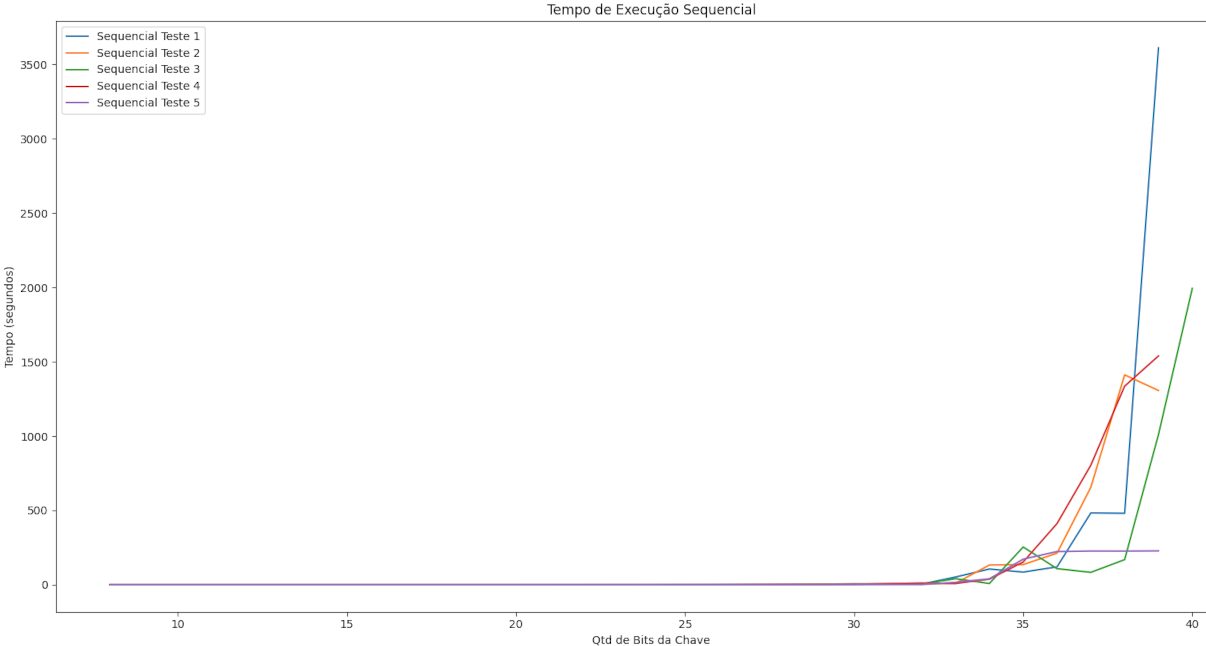
\includegraphics[scale=.42]{Figuras/TempoExecuçãoSerial1.png}
                \caption{Gráfico do Tempo de Execução Serial}
            \end{figure}
        \end{adjustwidth}
    \end{frame}

    \begin{frame}{Tempos de Execução Paralelos}
   
    \end{frame}

    \begin{frame}{Tempos Serial e Paralelo}
   
    \end{frame}

    \begin{frame}{Speed Up e Eficiência}
   
    \end{frame}

    \begin{frame}{Gráficos}

    \end{frame}
\end{document}